\documentclass[11pt]{article}
\usepackage[T1]{fontenc}
\usepackage{lmodern,microtype,amsmath,amssymb,mathrsfs,booktabs,array,graphicx}
\usepackage[margin=0.9in]{geometry}
\usepackage{xcolor}
\definecolor{teal}{HTML}{087E83}
\usepackage[colorlinks=true,linkcolor=teal,urlcolor=teal]{hyperref}
\usepackage{enumitem}
\setlist{itemsep=3pt,topsep=5pt}
\setlength{\parskip}{4pt}
\setlength{\parindent}{0pt}
\newcommand{\PP}{\mathbf P}
\newcommand{\Bl}{\operatorname{Bl}}
\newcommand{\kk}{\mathbf k}
\newcommand{\OO}{\mathcal O}
\title{Common projection centers\\\large Results, applications, and computational projects}
\author{A computational companion for Zixin Yu}
\date{September 12, 2026}
\begin{document}
\maketitle

\section{What the paper establishes}
The paper studies two general ordered configurations $X,Y$ of $N=d+3$ points in $\PP^d$, with $d\geq3$. It asks for all pairs of centers $(a,b)$ such that projecting $X$ from $a$ and $Y$ from $b$ gives projectively equivalent configurations in $\PP^{d-1}$. Centers equal to data points are excluded. The revised manuscript gives an embedded classification of the closure and a detailed description of its coordinate algebra.

\textbf{The solution space is a surface with two explicit parameters.} Each configuration matrix has a two-dimensional kernel. Its coordinate zeros give $N$ Gale points on a projective line. Pairing the two lists gives points $p_i$ on $Q=\PP^1\times\PP^1$, and the centers surface is
\[
S=\Bl_{p_1,\ldots,p_N}Q.
\]
The blow-up records approach directions at the parameters where the raw center formulas vanish. Thus the compactification has a concrete computational meaning.

\textbf{Both projections are balanced scrolls.} Writing $F_1,F_2$ for the ruling classes and $E_i$ for the exceptional curves, the two hyperplane classes are
\[
A=F_1+(d+1)F_2-\sum E_i,\qquad
B=(d+1)F_1+F_2-\sum E_i.
\]
Their images are $S(\lfloor(d-1)/2\rfloor,\lceil(d-1)/2\rceil)$. The first map contracts $C_i=F_2-E_i$ to $x_i$; the second contracts $D_i=F_1-E_i$ to $y_i$. The pair map embeds $S$ in $\PP^d\times\PP^d$. Every valid pair is covered, including most points on each $E_i$.

\textbf{The boundary is completely identified.} The valid locus is $S\setminus\bigcup_i(C_i\cup D_i)$. The boundary has $2(d+3)$ rational components and $(d+3)(d+2)$ transverse nodes. The logarithmic canonical divisor is ample. Its complex Euler characteristic is $(d+1)^2$. This Euler characteristic concerns the complex valid surface, not the real pictures in the viewer.

\textbf{The embedding has a precise algebraic defect.} Let $R$ be its bigraded coordinate ring and $\mathscr B=\bigoplus_{p,q\geq0}H^0(S,pA+qB)$ its full section algebra. Then
\[
0\longrightarrow R\longrightarrow\mathscr B\longrightarrow
\kk(-1,-1)^{d-1}\longrightarrow0.
\]
All nonnegative section dimensions are explicit. The only missing coordinate sections occur at $(1,1)$. The algebra $\mathscr B$ is the normalization, is Cohen--Macaulay of regularity two, and has the proved Betti table displayed in the lab. The original ring has regularity three, so its ideal is generated in total degree at most four. Its remaining mixed Betti numbers are still open.

\textbf{The geometry retains the configuration.} The two polarizations recover the original ruling classes and the marked paired Gale configuration. The marked family has dimension $2d$. This leads to the projective signature experiment below.

\section{How the theory can be used}
The strongest applications concern identifiability, constrained exact reconstruction, and computational algebra. The physical camera interpretation is most immediate for $d=3$. Higher dimensions describe abstract projective projection problems.

\subsection{Describe and generate exact ambiguities}
The surface gives a family of pairs of views that agree projectively. It can generate exact examples for testing whether an algorithm confuses distinct configurations, drops solutions near a base point, or silently treats a boundary center as valid. This is directly related to the common-image problem of Ottaviani--Thomas \cite{OT}; the broader projective-camera framework is described by Hartley--Zisserman \cite{HZ}.

The result assumes arbitrary projective image equivalence. A calibrated camera model, Euclidean pose, positive depth, visibility, and image-domain bounds impose additional restrictions. These must be added before treating a point of the algebraic surface as a physically admissible camera. The current projects concern exact projective geometry.

\subsection{Turn geometric constraints into finite candidate sets}
The multidegree is
\[
(A^2,AB,B^2)=(d-1,d^2+d-1,d-1).
\]
Consequently two general hyperplane conditions on the first center leave $d-1$ points; one on each center leaves $d^2+d-1$ points. These are complex intersection counts, with multiplicity. General choices avoid the boundary and are transverse in characteristic zero.

For $d=3$, a hyperplane is an ordinary projective plane in camera-center space. One plane constraint on each center generically leaves $11$ complex candidates. For $d=4$, the analogous count is $19$. This is a direct consequence of the paper and gives a finite exact reconstruction problem with a known answer count. It also supplies a stopping criterion for a solver, once multiplicities and boundary exclusion are handled.

\subsection{Create marked projective signatures}
Normalize the first three points in each Gale list to $\infty,0,1$. If the affine coordinates are $t_1,t_2,t_3,t$, the normalized coordinate is
\[
\frac{(t-t_2)(t_3-t_1)}{(t-t_1)(t_3-t_2)}.
\]
The remaining $d$ values from each factor give $2d$ rational invariants. They allow differently represented copies of the same marked data to be compared without constructing the full centers surface. The interpretation uses the projective Gale transform \cite{EP}. Labels matter; an unordered comparison would require a separate permutation problem.

\subsection{Use a structured benchmark for algebraic solvers}
The equations have a uniform degree bound, the normalized resolution is explicit, and mixed hyperplane sections have known degree. Together these give several independent checks for elimination and homotopy computations. Macaulay2 supports multigraded resolutions and Betti tables \cite{M2}; parameter homotopies provide a route for moving already-known solutions as constraints vary \cite{HC}.

Two concrete further research problems are to determine the ranks of the Tor maps controlling the unresolved resolution of $R$, and to determine the discriminant and real-root chambers of the constrained-center problem. The supplied code gives reproducible inputs for both. Neither problem is claimed solved by the visualizations.

\section{The delivered projects}
The browser companion is the single file \texttt{common\_centers\_lab.html}. Download it and open it in a browser. It has no external scripts, installation step, or data connection. Its three tabs share the same formulas and deterministic data.

\subsection{Project 1: center pairs and scrolls}
\textbf{Implemented:} examples in dimensions $3,4,5$; two Gale-parameter controls; clickable parameter square; rotatable scroll point clouds; fixed-center families $C_i,D_i$; full homogeneous coordinates; a projectivity $H$ matching the images; JSON export and a scroll-image export.

\textbf{Try this:} begin at $d=3$ and move either parameter. The images continue to coincide after the computed $H$. Then choose ``$C_i$: $a$ stays fixed.'' The first center collapses to $x_i$, while the second follows a degree-$d$ rational normal curve. The pair is now on the excluded boundary, and the interface identifies that change.

The cloud is an affine window in the real scroll. For $d>3$, its coordinates are linearly projected to three display coordinates. These shadows can cross. They do not display the full embedded surface or its complex topology.

\begin{figure}[ht]
\centering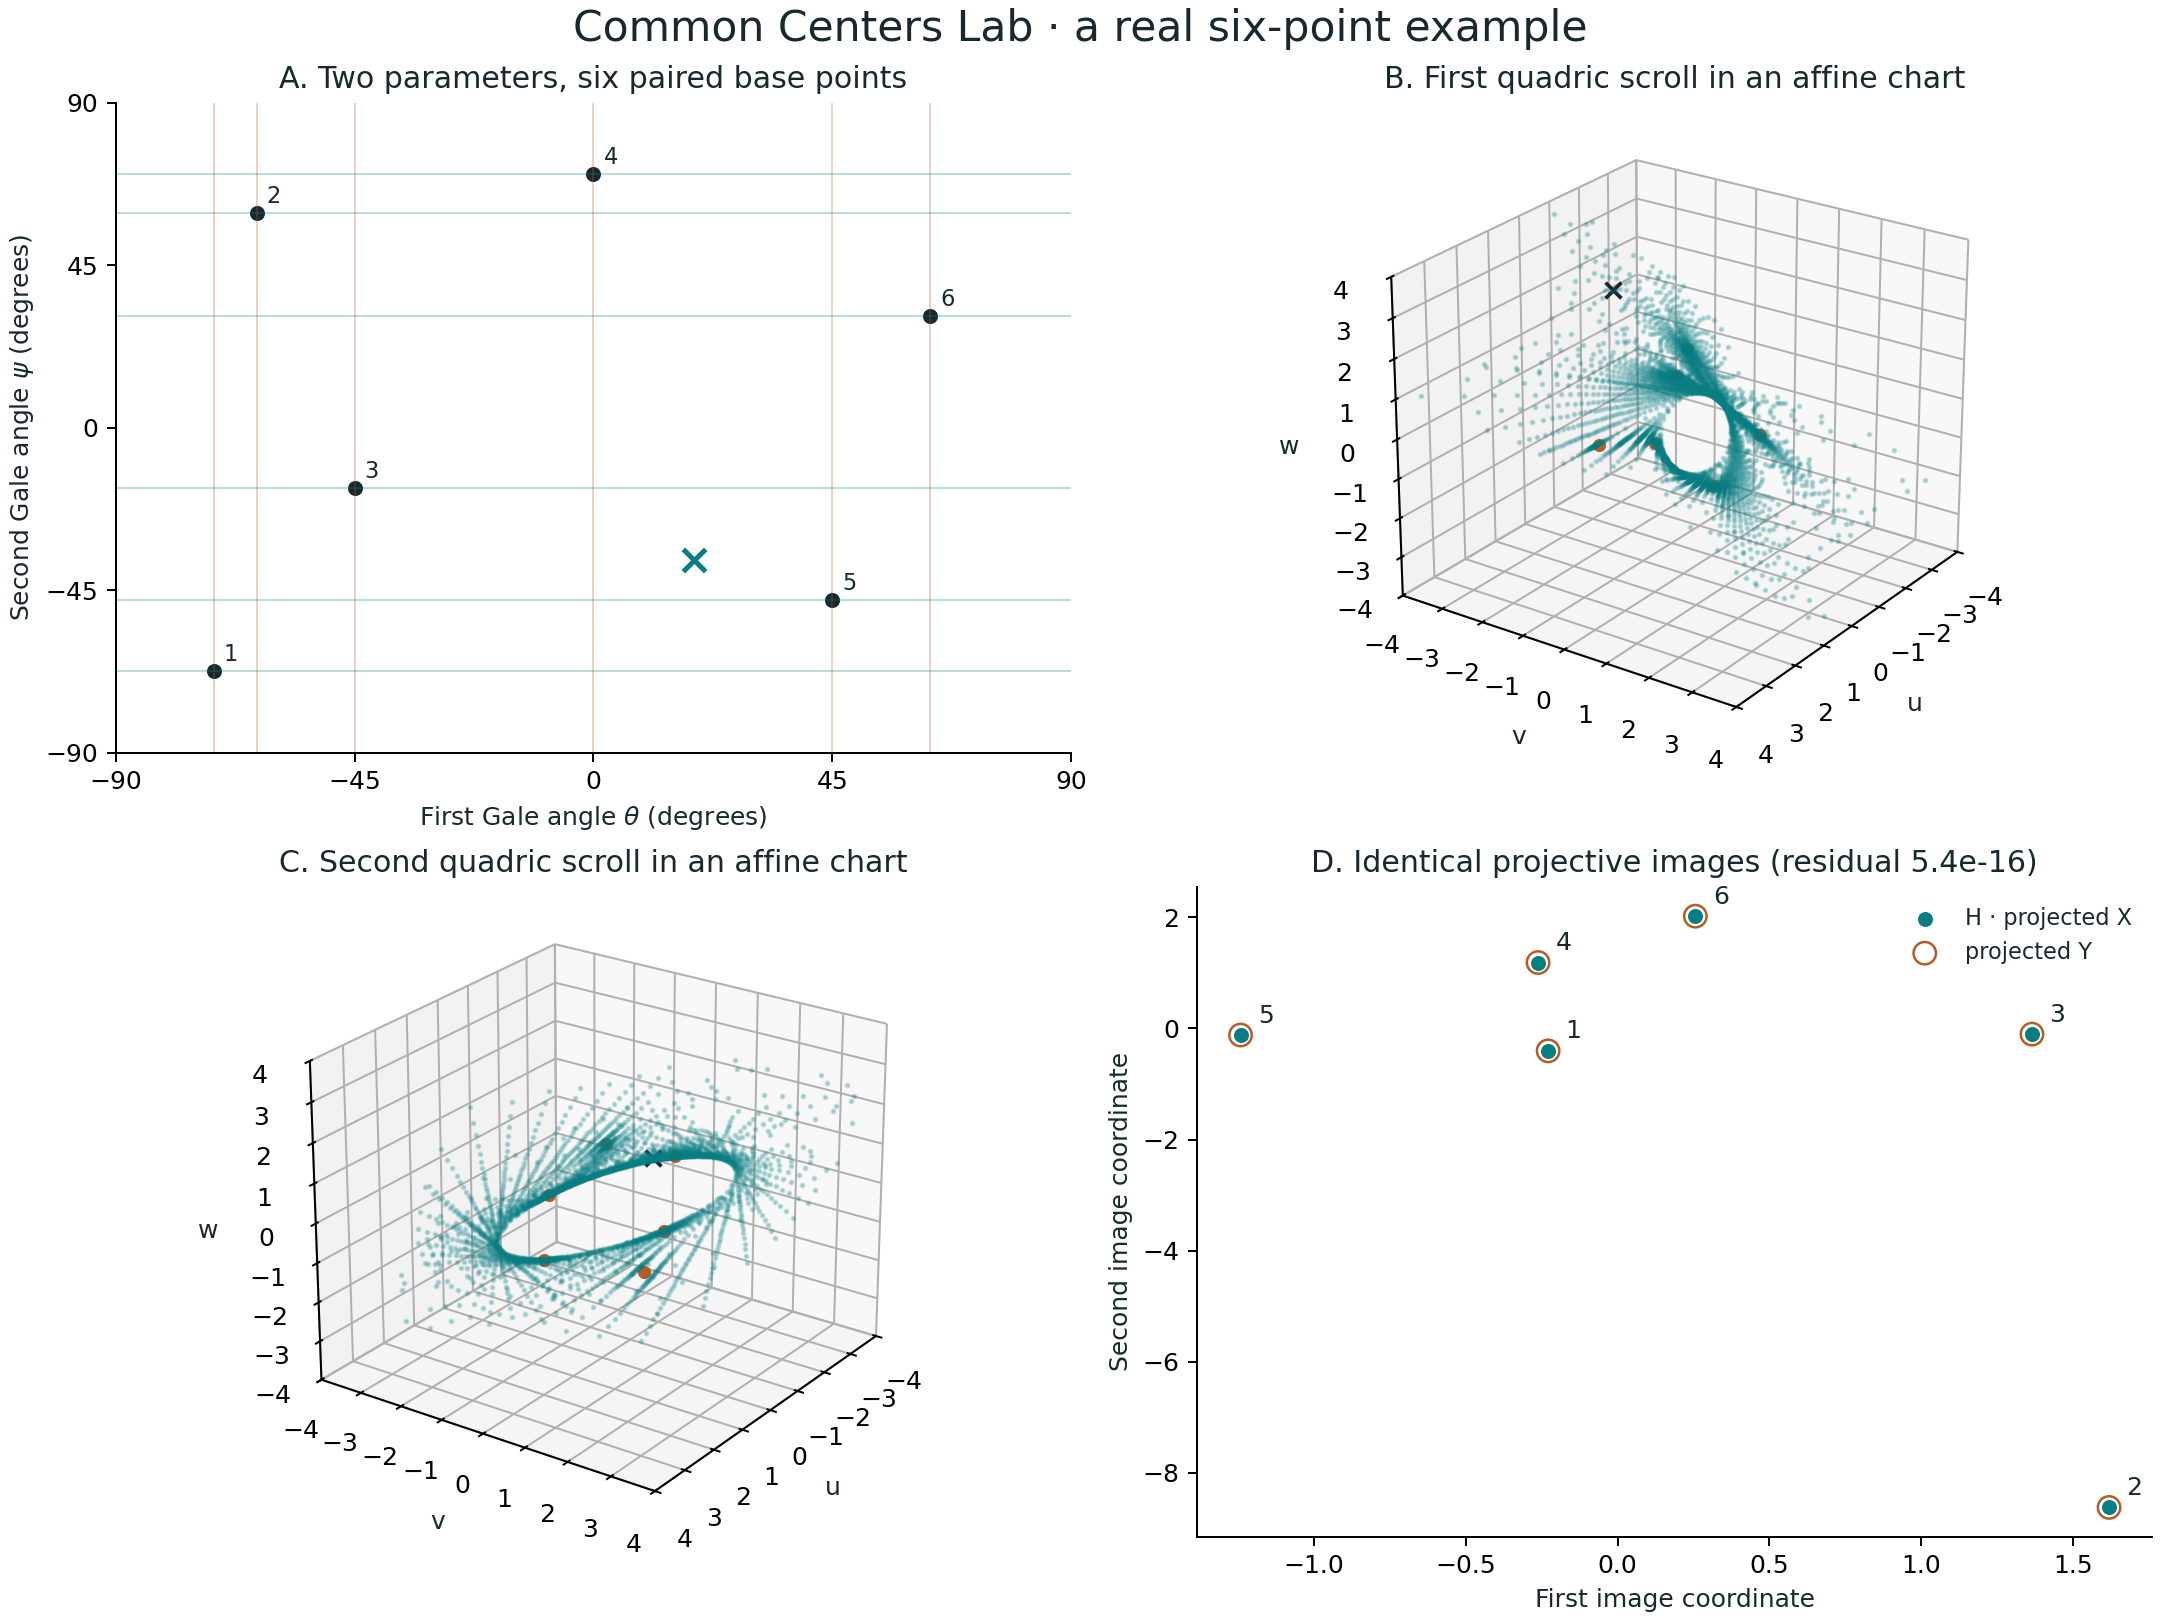
\includegraphics[width=\textwidth]{geometry_overview.png}
\caption{A real six-point example generated by the supplied code. The Gale parameters determine a point on each quadric scroll. The last panel independently computes the quotient cameras and the matching projectivity.}
\end{figure}

\subsection{Project 2: the blow-up microscope}
\textbf{Implemented:} every labeled $E_i$ for $d=3,4,5$; approach direction $[\cos\phi:\sin\phi]$; direct evaluation of the resolved limit in floating-point coordinates; a nearby-point mode with $\varepsilon$ from $10^{-1}$ to $10^{-6}$; boundary incidence cells that open the corresponding center pair; JSON export.

The coordinates near $p_i$ are $t=t_i+\varepsilon\cos\phi$, $s=s_i+\varepsilon\sin\phi$. The raw vectors are first order in $\varepsilon$. Their linear terms define the resolved centers on $E_i$ directly. This avoids choosing an arbitrary tiny radius to approximate the exceptional curve. The real exceptional curve is a circle, $\PP^1(\mathbf R)$; the complex curve is $\PP^1(\mathbf C)$.

\textbf{Try this:} at $d=4$, select $E_1$ and vary $\phi$ with ``On $E_i$'' selected. Most directions are valid. At $0^\circ$ the first center is a data point; at $90^\circ$ the second is a data point. Uncheck the limit mode and decrease $\varepsilon$ to see convergence to the resolved value.

\subsection{Project 3: the algebra and degree explorer}
\textbf{Implemented:} dimensions $3$ through $10$ for the Hilbert and Betti formulas; selectable bidegrees; the unique deficiency at $(1,1)$; multidegrees and Segre degrees; proved quadratic and cubic generator counts; the complete normalization Betti table; downloadable data.

The second half contains exact mixed-hyperplane examples in dimensions $3$ and $4$. The hyperplanes are expressed in the integer configuration matrices stored in the certificate. These matrices are projectively equivalent to the orthonormal matrices used for the geometry viewer.

\begin{center}
\begin{tabular}{@{}rrrrrr@{}}
\toprule
$d$ & Raw eliminant degree & Base factors & Valid complex pairs & Real & Nonreal\\
\midrule
3 & 17 & 6 & 11 & 9 & 2\\
4 & 26 & 7 & 19 & 9 & 10\\
\bottomrule
\end{tabular}
\end{center}

These counts are for the stated rational examples. The eliminant is divided by the $N$ known base factors exactly. The residual polynomial has the expected degree, is squarefree, and is coprime to the denominator and the base factors. A Sturm sequence certifies its real-root count. Only the locations of the plotted roots use floating-point arithmetic. In the $d=4$ example, all $19$ roots give distinct valid complex center pairs, of which exactly $9$ are real.

\begin{figure}[ht]
\centering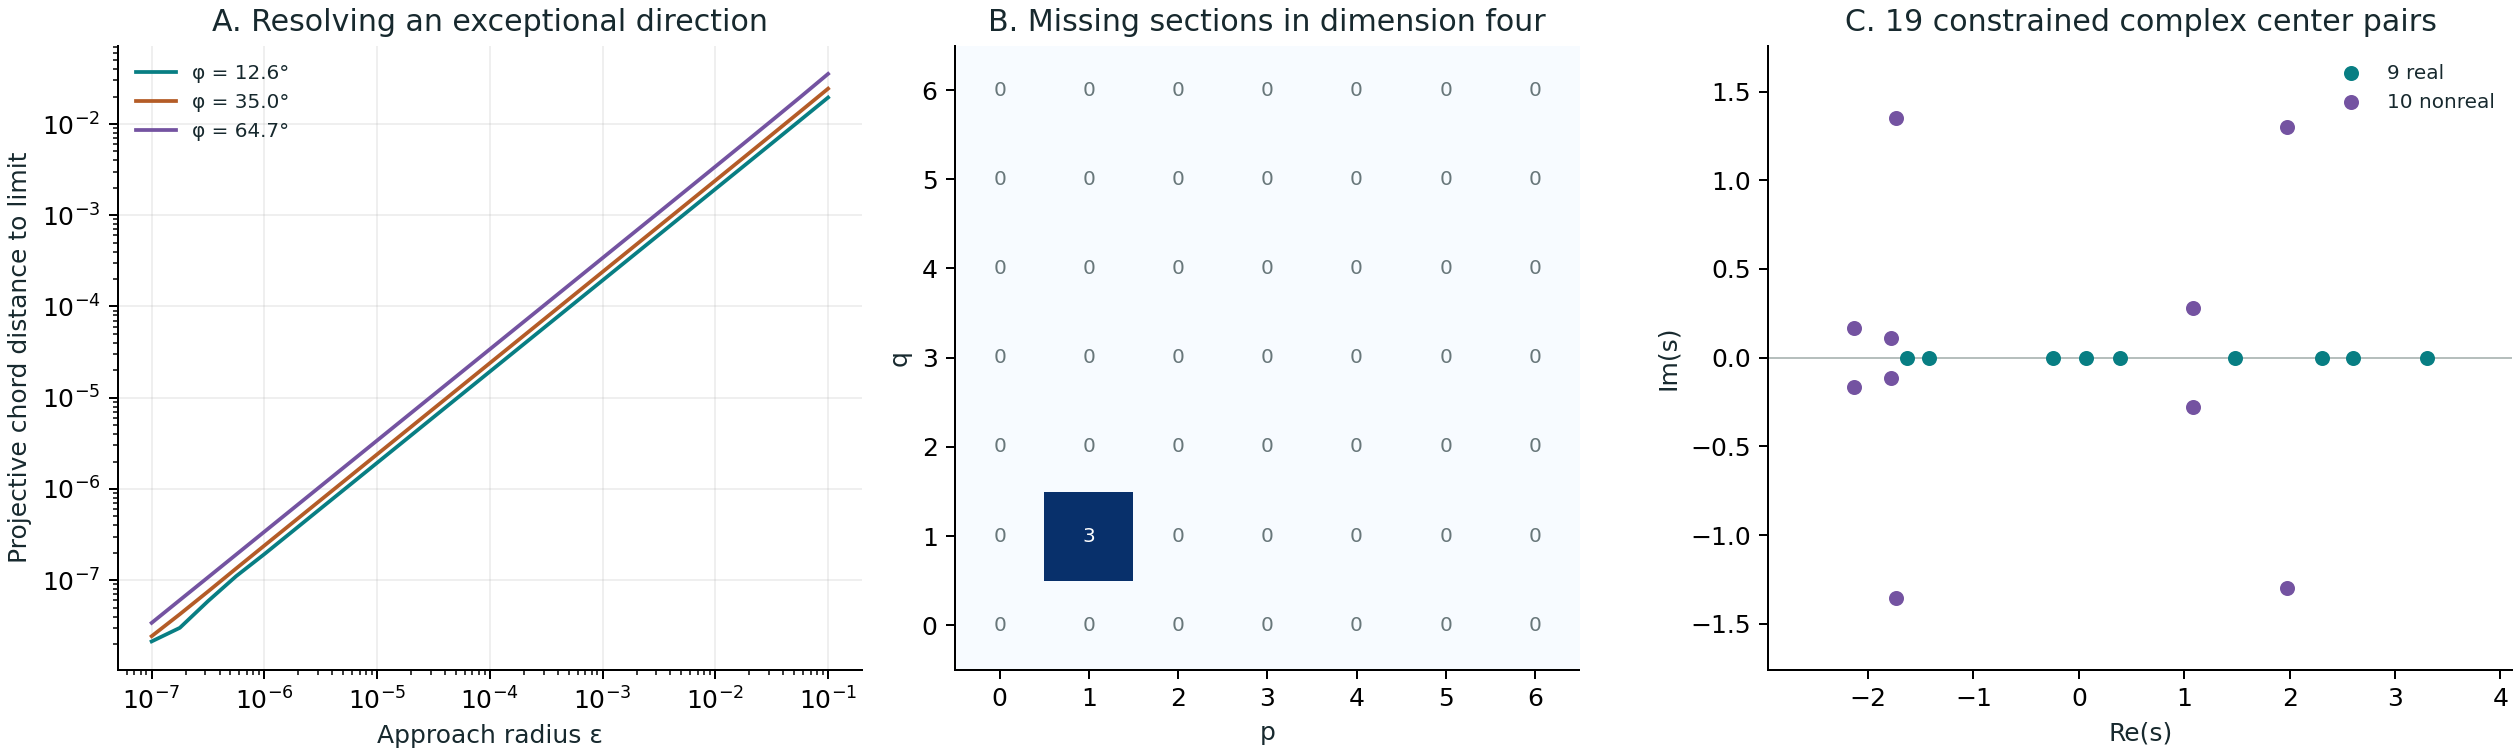
\includegraphics[width=\textwidth]{algebra_and_boundary.png}
\caption{Three computed manifestations of the theory in dimension four: approach to an exceptional direction; the unique three-dimensional deficiency of the coordinate ring; and the mixed hyperplane section with nine real and ten nonreal points.}
\end{figure}

\subsection{Companion notebook and exact signature module}
The notebook \texttt{common\_centers\_experiments.ipynb} contains six executed code cells. It reconstructs the matching projectivity, resolves a base point, evaluates section and Betti formulas, certifies the $19$-point example, and computes the eight marked projective invariants for $d=4$. It includes its outputs and figures.

The module \texttt{gale\_signature.py} verifies with rational arithmetic that two independently chosen projectivities preserve those invariants. The files \texttt{geometry.py}, \texttt{algebra.py}, and \texttt{slice\_exact.py} expose the underlying functions for further experiments. In \texttt{slice\_instance(d, seed=...)}, changing the seed chooses new rational hyperplanes for the same configuration.

\section{Reproduction and validation}
Extract the package and run from its folder:
\begin{verbatim}
python3 -m pip install -r requirements.txt
python3 run_all.py
python3 make_figures.py
python3 build_notebook.py
node test_engine.js
node test_ui.js
\end{verbatim}
The browser file itself requires none of these steps. They rebuild the data, formulas, static figures, notebook, and offline explorer. Node is needed only for the two developer tests.

The Python geometry checks cover ordinary parameters, every exceptional curve, both contraction families, and convergence to the resolved limit. Across the included examples, the tested ordinary and exceptional matching residuals are below $10^{-13}$. A separate JavaScript check covers $219$ ordinary and exceptional parameter cases; its largest residual is $2.21\times10^{-14}$. Exact rational interpolation checks confirm the balanced splitting ranks for the displayed data.

The Hilbert/Betti implementation reconstructs section dimensions from its alternating free-module sum for $d=3,\ldots,10$. This is an arithmetic consistency check on the proved formulas. The slice degree, squarefreeness, coprimality, and real-root counts are independently checked over $\mathbf Q$.

The actual interface handlers were exercised in a DOM/canvas stand-in: $133$ state checks, including exceptional endpoints and boundary-cell navigation. A browser executable was unavailable in the build environment, so a full browser layout test was not completed. The static scientific figures and this PDF were rendered and visually inspected. Source files are included so every computation and display convention is reviewable.

\begin{thebibliography}{9}\raggedright
\bibitem{OT} G. Ottaviani and R. R. Thomas, \emph{When is one pinhole camera image equal to some other pinhole camera image?} (2026), \url{https://arxiv.org/abs/2603.14172}.
\bibitem{EP} D. Eisenbud and S. Popescu, \emph{The Projective Geometry of the Gale Transform}, J. Algebra 230 (2000), 127--173. Preprint: \url{https://arxiv.org/abs/math/9807127}.
\bibitem{HZ} R. Hartley and A. Zisserman, \emph{Multiple View Geometry in Computer Vision}, 2nd ed., Cambridge University Press, 2004. Authors' page: \url{https://www.robots.ox.ac.uk/~vgg/hzbook/}.
\bibitem{M2} Macaulay2 documentation, \emph{MultigradedBettiTally}. \href{https://macaulay2.com/doc/Macaulay2/share/doc/Macaulay2/Macaulay2Doc/html/___Multigraded__Betti__Tally.html}{Official multigraded Betti-table documentation}.
\bibitem{HC} HomotopyContinuation.jl documentation, \emph{Systems with parameters}. \url{https://www.juliahomotopycontinuation.org/guides/parameter-homotopies/}.
\end{thebibliography}
\end{document}
